\setcounter{page}{1} \pagenumbering{Alph}

% Add PDF bookmark 
\pdfbookmark[0]{Title}{Title}

\thispagestyle{empty}

\begin{flushleft} ~\\ \vspace{-12mm} \hspace{-12mm}

\includegraphics[width=50mm]{Cover/istnewlogo}
\vspace{10mm}
%~\\ \vspace{50mm} % gráficos
\\ \begin{center} 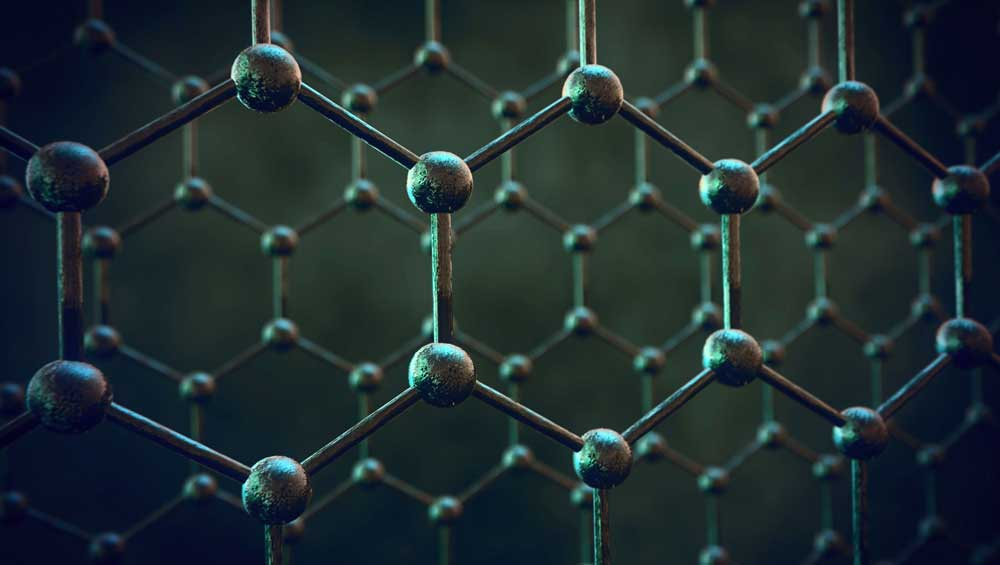
\includegraphics[height=50mm]{Cover/coverimage} \end{center} % gráficos
 \vspace{5mm}
\centering
\LARGE \textbf{Development of a QMC code to tackle interacting electronic systems in 2D with application to TMD nanoribbons}
\\
\vspace{15mm}
\Large \textbf{Francisco Monteiro de Oliveira Brito} \\
\vspace{12mm}
\large Thesis to obtain the Master of Science Degree in
\\ \vspace{2mm}
\LARGE \textbf{Physics Engineering}
\\ \vspace{10mm}
\large Supervisor(s): Prof. Eduardo Filipe Vieira de Castro  \\
\large Prof. João Manuel Viana Parente Lopes 
\\ \vspace{10mm}
\Large \textbf{Examination Committee}
\\ \vspace{5mm}
\large Chairperson: Prof. Pedro Domingos Santos do Sacramento \\
\large Supervisor: Prof. Eduardo Filipe Vieira de Castro \\
\large Co-Supervisor: Prof. João Manuel Viana Parente Lopes  \\
\large Members of the Committee: Prof. Pedro José Gonçalves Ribeiro \\
%\vspace{15mm}
\vspace{5mm}
\Large \textbf{\todaythesis\today} \\
\let\thepage\relax
\end{flushleft}
\pagebreak


\clearpage
% Since I am using double sided pages, the second page should be white.
% Remember that when delivering the dissertation, IST requires for the cover to appear twice.

\thispagestyle{empty}
\cleardoublepage

\setcounter{page}{1} \pagenumbering{roman}

\baselineskip 18pt % line spacing: -12pt for single spacing
                   %               -18pt for 1 1/2 spacing
                   %               -24pt for double spacingnts}
